\begin{frame}{Generalized linear model}
    \begin{tikzpicture}[remember picture,overlay]
        \begin{scope}[xshift=0.5\textwidth]
            \node (feature) at (-3.5,3) {$\dici{} \sim \mathcal{A}$};
            \node at ($(feature.north)+(0,0.2)$) {\textcolor{mLightBrown}{Features in $\kR^{\pdim}$}};
            %
            \node (outcome) at (3.5,3) {$\obsi{} \sim \phi(\transp{\dici{}}\pv)$};
            \node at ($(outcome.north)+(0,0.2)$) {\textcolor{mLightBrown}{Outcome in $\kR$}};
            %
            \draw[ultra thick,->] (feature) -- (outcome) node[midway,above] {weights $\pv \in \kR^{\pdim}$} node[midway,below] {link function $\kfuncdef{\phi}{\kR^{\pdim}}{\kR}$};
            %
            %
            %
            \node[very thick] (cell) at (0, 0.75) {};
            \node[very thick] at ($(cell)+(0,0.3)$) {\small{Cell}};
            \draw[very thick] (cell) ellipse (1cm and 0.8cm);
            \draw[very thick, dashed] (cell) ellipse (1.1cm and 0.9cm);
            \node[very thick] at ($(cell)+(0,-0.2)$) {\small{$\phi(\transp{\dici{}}\pv)$}};
            %
            \node (gene1) at ($(cell)+(-3,1)$) {\small{Gene 1}};
            \node (gene2) at ($(gene1)+(0,-0.75)$) {\small{Gene 2}};
            \node at ($(cell)+(-3,-0.4)$) {...};
            \node (genen) at ($(cell)+(-3,-1)$) {\small{Gene $\pdim$}};
            %
            \draw[very thick,->] (gene1.east) -- ($(cell)+(-1.1,0.5)$) node[midway,above] {$\dicii{1}$};
            \draw[very thick,->] (gene2.east) -- ($(cell)+(-1.25,0.15)$) node[midway,above] {$\dicii{2}$};
            \draw[very thick,->] (genen.east) -- ($(cell)+(-1.1,-0.5)$) node[midway,above] {$\dicii{n}$};
            %
            \node at ($(gene1.west)+(-0.2,0.3)$) {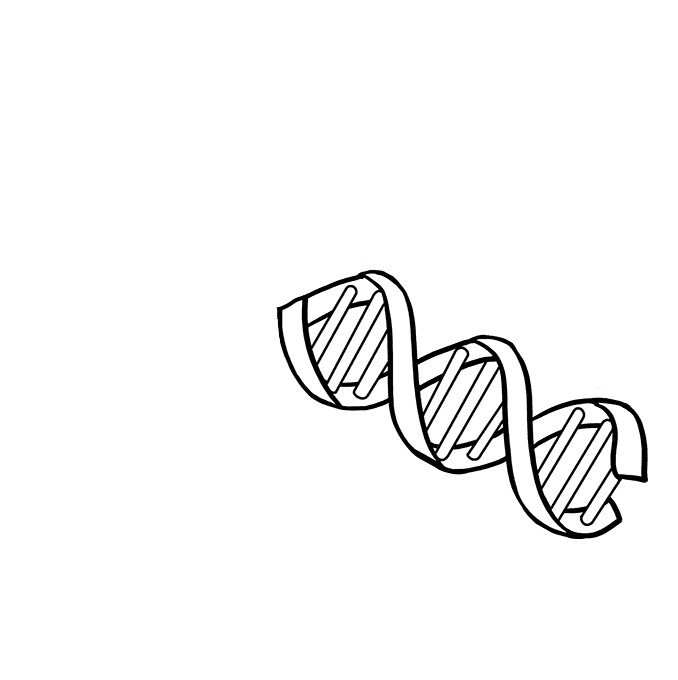
\includegraphics[width=30pt,angle=-60]{img/dna.png}};
            \node at ($(gene2.west)+(-0.2,0.3)$) {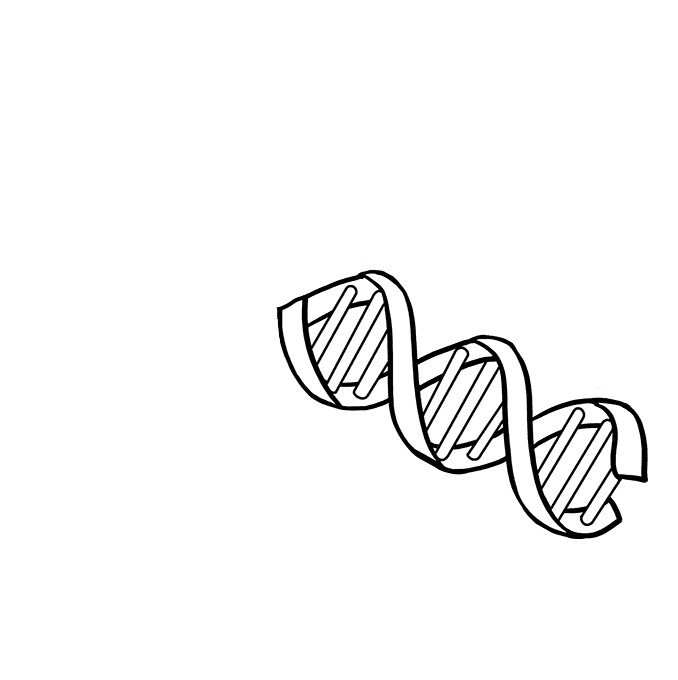
\includegraphics[width=30pt,angle=-60]{img/dna.png}};
            \node at ($(genen.west)+(-0.2,0.3)$) {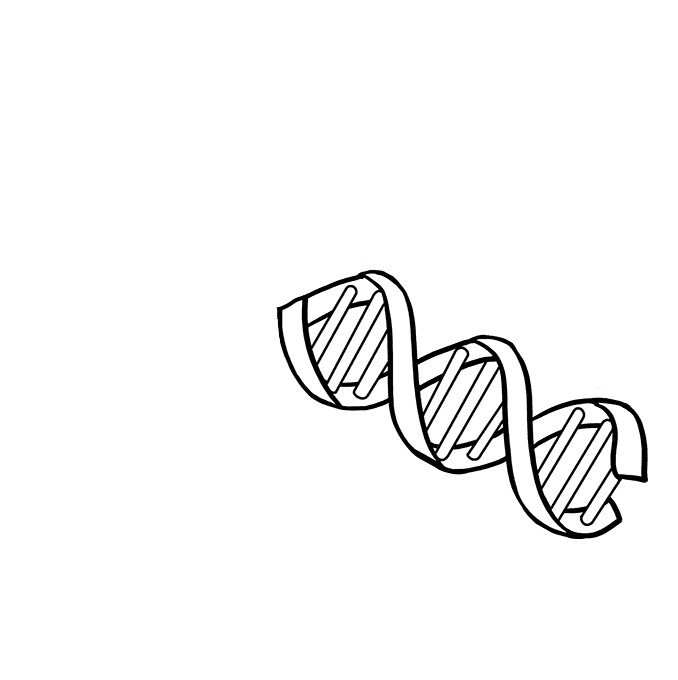
\includegraphics[width=30pt,angle=-60]{img/dna.png}};
            %
            \draw[very thick, ->] ($(cell)+(1.2,0)$) -- ($(cell)+(2.7,0)$) node[midway,above] {$\obsi{}$};
            \draw[very thick] ($(cell)+(3.5,-0.15)$) -- ++(90:0.3) -- ++(150:0.3) -- ++(210:0.3) -- ++(270:0.3) -- ++(330:0.3) -- cycle;
            \draw[very thick] ($(cell)+(3.5,-0.15)$) -- ++(330:0.3);
            \draw[very thick] ($(cell)+(3.5,-0.15)+(90:0.3)$) -- ++(30:0.3);
            \draw[very thick] ($(cell)+(3.5,-0.15)+(-0.5,0)$) -- ++(210:0.3);
            \node at ($(cell)+(3.25,-0.75)$) {\small{Protein production}};
            %
            %
            %
            \node[draw,ultra thick] (question) at (0,-1.5) {What is the importance of each feature on the outcome ?};
            %
            \node[align=center,text width=0.5\textwidth] (erm) at ($(question)+(0,-1.5)$) {
            \begin{blockcolor}{black}{Expected risk minimization}
                \centering
                $\min_{\pv \in \kR^{\pdim}} \mathbb{E}_{\dici{} \sim \mathcal{A}}[\mathcal{L}(\transp{\dici{}}\pv,\obsi{})]$
            \end{blockcolor}
            };
            % 
            \draw[ultra thick,->] (question) -- ($(erm)+(0,0.45)$) node[midway,right] {Loss $\mathcal{L}$};
        \end{scope}
    \end{tikzpicture}
\end{frame}
  
\begin{frame}{Sparse expected risk minimization}
    \begin{tikzpicture}[remember picture,overlay]
        \begin{scope}[xshift=0.5\textwidth]
            \node[text width=0.45\linewidth, align=center] (sample-text) at (-3,1.75) {\textbf{Unknown distribution $\mathcal{A}$}};
            %
            \node[text width=0.45\linewidth, align=center] (sparse-text)at (3,1.75) {\textbf{Few relevant features}};
            %
            \node (table) at (0,-0.5) {
                \scriptsize
                \begin{tabular}{c|cccccc|c}
                    \multicolumn{8}{c}{\small{Riboflavin dataset - P. Bühlmann \textit{et al.} (2014)}} \\
                    \toprule
                    Colony & \textcolor{mLightBrown}{AADK} & AAPA & \textcolor{mLightBrown}{ABFA} & ABH & ... & ZUR & \textbf{B2 prod.} \\
                    \midrule
                    \#1 & 8.49 & 8.11 & 8.32 & 10.28 & ... & 7.42 & \textbf{-6.64} \\
                    \#2 & 7.63 & 7.23 & 7.28 & 9.86 & ... & 7.54 & \textbf{-6.94} \\
                    \#3 & 8.08 & 7.85 & 7.79 & 9.67 & ... & 7.71 & \textbf{-7.93} \\
                    \#4 & 7.88 & 7.93 & 7.99 & 9.68 & ... & 7.26 & \textbf{-8.28} \\
                    ... & ... & ... & ... & ... & ... & ... \\
                    \#71 & 6.85 & 8.27 & 7.98 & 8.04 & ... & 6.65 & \textbf{-7.58} \\
                    \bottomrule
                \end{tabular}
            };
            %
            \draw[ultra thick,->] ($(sample-text.south)+(-1.5,0)$) .. controls ($(table.west)+(-1.25,1)$) .. (table.west) node [midway,fill=mLightWhite,draw,ultra thick,font=\scriptsize,text width=0.125\linewidth,align=center] {\small{Samples $\{\dici{j},\obsi{j}\}_{j=1}^{\ddim}$}};
            %
            \draw[ultra thick,->] ($(sparse-text.south)+(1.5,0)$) .. controls ($(table.east)+(1.25,1)$) .. (table.east) node [midway,fill=mLightWhite,draw,ultra thick,font=\scriptsize,text width=0.125\linewidth,align=center] {\small{$\ell_0$-norm $\norm{\pv}{0}$}};
            %
            \node[align=center,text width=0.55\textwidth] (erm) at (0,3.25) {
                \begin{blockcolor}{black}{Expected risk minimization}
                    \centering
                    $\min_{\pv \in \kR^{\pdim}} \mathbb{E}_{\dici{} \sim \mathcal{A}}[\mathcal{L}(\transp{\dici{}}\pv,\obsi{})]$
                \end{blockcolor}
            };
            %
            \node[align=center,text width=0.55\textwidth] (serm) at (0,-3) {
            \begin{blockcolor}{black}{Sparse empirical risk minimization}
                \centering
                $\min_{\pv \in \kR^{\pdim}} \ \tfrac{1}{\ddim}\sum_{j=1}^{\ddim}\mathcal{L}(\transp{\dici{j}}\pv,\obsi{j}) + \reg\norm{\pv}{0}$
            \end{blockcolor}
            };
        \end{scope}
    \end{tikzpicture}
\end{frame}
  
\begin{frame}{The problem of interest}
    \begin{tikzpicture}[remember picture,overlay]
        \begin{scope}[xshift=0.5\textwidth]
            \node[align=center,text width=0.5\textwidth] (problem) at (0,3.25) {
            \begin{blockcolor}{black}{$\boldsymbol{\ell}_0$-regularized problem}
                \centering
                $\min_{\pv \in \kR^{\pdim}} \lfunc(\dic\pv) + \reg\norm{\pv}{0} + \pfunc(\pv)$
            \end{blockcolor}
            };
        \end{scope}
        \begin{scope}[xshift=0.5\textwidth,yshift=40,scale=0.7,every node/.style={font=\scriptsize}]
            \path[mindmap,concept color=mLightBrown, level 1 concept/.append style={minimum size=1.2cm,text width=1.2cm,level distance=4.5cm,sibling angle=60}, level 2 concept/.append style={minimum size=1cm,text width=1cm,level distance=2.5cm}]
            node[concept,text=white,minimum size=1.6cm,text width=1.6cm] {\textbf{$\boldsymbol{\ell}_0$-regularized problems}}
            [clockwise from=0]
            child[concept color=blue!60!green!30] {
            node[concept] {\textbf{signal processing}}
            [clockwise from=60]
            child { node[concept] {denoising} }
            child { node[concept] {sparse decoding} }
            child { node[concept] {phase retrieval} }
            child { node[concept] {DOA design} }
            }  
            child[concept color=red!40] {
            node[concept] {\textbf{operation research}}
            [clockwise from=340]
            child { node[concept] {portfolio optim.} }
            child { node[concept] {network design} }
            }
            child[concept color=yellow!50!red!30] { node[concept] {\textbf{algebra}}
            [clockwise from=330]
            child { node[concept] {matrix factor.} }
            child { node[concept] {matroid} }
            child { node[concept] {max feasible system} }
            }
            child[concept color=green!80!blue!30] { node[concept] {\textbf{statsistics \& ML}} 
            [clockwise from=300]
            child { node[concept] {sparse PCA} }
            child { node[concept] {sparse SVMs} }
            child { node[concept] {dictionary learning} }
            child { node[concept] {feature selection} }
            };
        \end{scope}
        \node at (0.5\textwidth,-4) {\scriptsize{A. Tillman, D. Bienstock, A. Lodi, A. Schwartz (2024)}};
    \end{tikzpicture}
\end{frame}
  
\begin{frame}{A bit of history}
    \begin{tikzpicture}[remember picture,overlay]
        \begin{scope}[xshift=0.5\textwidth]
            \node[align=center,text width=0.5\textwidth] (problem) at (0,3.25) {
            \begin{blockcolor}{black}{$\boldsymbol{\ell}_0$-regularized problem}
                \centering
                $\min_{\pv \in \kR^{\pdim}} \lfunc(\dic\pv) + \reg\norm{\pv}{0} + \pfunc(\pv)$
            \end{blockcolor}
            };
            %
            \node[mLightBrown,draw,ultra thick] (nphard) at ($(problem)+(0,-1.75)$) {\textcolor{mLightBrown}{NP-hard}};
            \draw[ultra thick,->] (problem) -- ($(nphard)+(0,0.35)$);
            %
            %
            %
            \node (linecenter) at ($(current page.north)+(0,-0.6\textheight)$) {};
            \draw [ultra thick,->] ($(linecenter)+(-6,0)$) -- ($(linecenter)+(6,0)$) node (arrow) [midway] {};
            %
            \node (date1) at ($(linecenter)+(-5,0)$) {};
            \draw [ultra thick,-] ($(date1)+(0,-0.02\textheight)$) -- ($(date1)+(0,0.02\textheight)$);
            \node at ($(date1)+(0,+0.06\textheight)$)  {\textbf{1990}};
            \node[text width=0.2\textwidth,align=center,font=\small] at ($(date1)+(0,-0.05\textheight)$) {Heuristics};
            \node[text width=0.3\textwidth,align=center,font=\scriptsize] at ($(date1)+(0,-0.12\textheight)$) {MP, OMP, \\ IHT, ...};
            %
            \node (origin1) at ($(date1)+(0,-0.4\textheight)$) {};
            \fill[draw,thick,fill=mLightWhite] ($(origin1)+(-0.5,0)$) circle (0.1);
            \fill[draw,thick,fill=mLightBrown] ($(origin1)+(-0.5,0.3)$) circle (0.1);
            \fill[draw,thick,fill=mLightWhite] ($(origin1)+(-0.5,0.6)$) circle (0.1);
            \fill[draw,thick,fill=mLightWhite] ($(origin1)+(-0.5,0.9)$) circle (0.1);
            \fill[draw,thick,fill=mLightWhite] ($(origin1)+(-0.5,1.2)$) circle (0.1);
            \fill[draw,thick,fill=mLightWhite] ($(origin1)+(-0.5,1.5)$) circle (0.1);
            \node at ($(origin1)+(-0.5,-0.4)$) {$\pv^1$};
            %
            \fill[draw,thick,fill=mLightWhite] ($(origin1)+(0,0)$) circle (0.1);
            \fill[draw,thick,fill=mLightBrown] ($(origin1)+(0,0.3)$) circle (0.1);
            \fill[draw,thick,fill=mLightWhite] ($(origin1)+(0,0.6)$) circle (0.1);
            \fill[draw,thick,fill=mLightBrown] ($(origin1)+(0,0.9)$) circle (0.1);
            \fill[draw,thick,fill=mLightWhite] ($(origin1)+(0,1.2)$) circle (0.1);
            \fill[draw,thick,fill=mLightWhite] ($(origin1)+(0,1.5)$) circle (0.1);
            \node at ($(origin1)+(0,-0.4)$) {$\pv^2$};
            %
            \fill[draw,thick,fill=mLightWhite] ($(origin1)+(0.5,0)$) circle (0.1);
            \fill[draw,thick,fill=mLightBrown] ($(origin1)+(0.5,0.3)$) circle (0.1);
            \fill[draw,thick,fill=mLightWhite] ($(origin1)+(0.5,0.6)$) circle (0.1);
            \fill[draw,thick,fill=mLightBrown] ($(origin1)+(0.5,0.9)$) circle (0.1);
            \fill[draw,thick,fill=mLightBrown] ($(origin1)+(0.5,1.2)$) circle (0.1);
            \fill[draw,thick,fill=mLightWhite] ($(origin1)+(0.5,1.5)$) circle (0.1);
            \node at ($(origin1)+(0.5,-0.4)$) {$\pv^3$};
            %
            %
            %
            \node (date2) at ($(linecenter)+(-2.5,0)$) {};
            \draw [ultra thick,-] ($(date2)+(0,-0.02\textheight)$) -- ($(date2)+(0,0.02\textheight)$);
            \node at ($(date2)+(0,+0.06\textheight)$)  {\textbf{2000}};
            \node[text width=0.25\textwidth,align=center,font=\small] at ($(date2)+(0,-0.053\textheight)$) {Recovery cond.};
            \node[text width=0.3\textwidth,align=center,font=\scriptsize] at ($(date2)+(0,-0.12\textheight)$) {RIP, NSP, \\ EkR, ...};
            %
            \node (origin2) at ($(date2)+(0,-0.4\textheight)$) {};
            \node at ($(origin2)+(0,0.12\textheight)$) {OMP};
            \node at ($(origin2)+(0,0.02\textheight)$) {$\ell_0$-problem};
            \node[rotate=90] at ($(origin2)+(0,0.07\textheight)$) {$\equiv$};
            %
            %
            %
            \node (date3) at ($(linecenter)+(0,0)$) {};
            \draw [ultra thick,-] ($(date3)+(0,-0.02\textheight)$) -- ($(date3)+(0,0.02\textheight)$);
            \node at ($(date3)+(0,+0.06\textheight)$)  {\textbf{2005}};
            \node[font=\small] at ($(date3)+(0,-0.053\textheight)$) {Convex approx.};
            \node[text width=0.3\textwidth,align=center,font=\scriptsize] at ($(date3)+(0,-0.12\textheight)$) {Lasso, Elastic-Net, \\ Hubert, ...};
            %
            \node (origin3) at ($(date3)+(0,-0.4\textheight)$) {};
            \draw[ultra thick,->] ($(origin3)+(-1,0)$) -- ($(origin3)+(1, 0)$);
            \draw[ultra thick,->] ($(origin3)+(0,0)$) -- ($(origin3)+(0,1.5)$);
            \draw[-,very thick,mLightBrown] ($(origin3)+(-0.05,0.8)$) -- ($(origin3)+(-1,0.8)$);
            \draw[-,very thick,mLightBrown] ($(origin3)+(0.05,0.8)$) -- ($(origin3)+(1,0.8)$);
            \draw[very thick,dashed,mLightBrown] (origin3) .. controls ($(origin3)+(-0.5,0.1)$) ..  ($(origin3)+(-1,0.8)$);
            \draw[very thick,dashed,mLightBrown] (origin3) .. controls ($(origin3)+(0.5,0.1)$) ..  ($(origin3)+(1,0.8)$);
            \draw[mLightBrown,very thick] ($(origin3)+(0,0.8)$) circle (0.075);
            \fill[mLightBrown] (origin3) circle (0.075);
            %
            %
            %
            \node (date4) at ($(linecenter)+(2.5,0)$) {};
            \draw [ultra thick,-] ($(date4)+(0,-0.02\textheight)$) -- ($(date4)+(0,0.02\textheight)$);
            \node at ($(date4)+(0,+0.06\textheight)$)  {\textbf{2010}};
            \node[font=\small] at ($(date4)+(0,-0.053\textheight)$) {Concave approx.};
            \node[text width=0.3\textwidth,align=center,font=\scriptsize] at ($(date4)+(0,-0.12\textheight)$) {SCAD, MCP, \\ CEL0, ...};
            %
            \node (origin4) at ($(date4)+(0,-0.4\textheight)$) {};
            \draw[ultra thick,->] ($(origin4)+(-1,0)$) -- ($(origin4)+(1, 0)$);
            \draw[ultra thick,->] ($(origin4)+(0,0)$) -- ($(origin4)+(0,1.5)$);
            \draw[-,very thick,mLightBrown] ($(origin4)+(-0.05,0.8)$) -- ($(origin4)+(-1,0.8)$);
            \draw[-,very thick,mLightBrown] ($(origin4)+(0.05,0.8)$) -- ($(origin4)+(1,0.8)$);
            \draw[very thick,mLightBrown,dashed] (origin4) .. controls ($(origin4)+(-0.5,0.8)$) ..  ($(origin4)+(-1,0.8)$);
            \draw[very thick,mLightBrown,dashed] (origin4) .. controls ($(origin4)+(0.5,0.8)$) ..  ($(origin4)+(1,0.8)$);
            \draw[mLightBrown,very thick] ($(origin4)+(0,0.8)$) circle (0.075);
            \fill[mLightBrown] (origin4) circle (0.075);
            %
            %
            %
            \node (date5) at ($(linecenter)+(5,0)$) {};
            \draw[ultra thick,-] ($(date5)+(0,-0.02\textheight)$) -- ($(date5)+(0,0.02\textheight)$);
            \node at ($(date5)+(0,+0.06\textheight)$)  {\textbf{2015}};
            \node[text width=0.22\textwidth,align=center,font=\small,mLightBrown] at ($(date5)+(0,-0.05\textheight)$) {Exact methods};
            \node[text width=0.3\textwidth,align=center,font=\scriptsize] at ($(date5)+(0,-0.12\textheight)$) {D. Bertsimas, A. King, R. Mazumder (2016)};
            %
            \node (origin5) at ($(date5)+(0,-0.4\textheight)$) {};
            \draw[ultra thick,->] ($(origin5)+(-1,0)$) -- ($(origin5)+(1, 0)$);
            \draw[ultra thick,->] ($(origin5)+(0,0)$) -- ($(origin5)+(0,1.5)$);
            \draw[-,very thick,mLightBrown] ($(origin5)+(-0.05,0.8)$) -- ($(origin5)+(-1,0.8)$);
            \draw[-,very thick,mLightBrown] ($(origin5)+(0.05,0.8)$) -- ($(origin5)+(1,0.8)$);
            \draw[mLightBrown,very thick] ($(origin5)+(0,0.8)$) circle (0.075);
            \fill[mLightBrown] (origin5) circle (0.075);
        \end{scope}
    \end{tikzpicture}
\end{frame}
  
\begin{frame}{Balancing quality and hardness}
    \begin{tikzpicture}[remember picture,overlay]
        \begin{scope}[xshift=0.5\textwidth]
            \node (dataset) at (0,2.5) {
                \scriptsize
                \begin{tabular}{c|cccccc|c}
                    \multicolumn{8}{c}{\small{Riboflavin dataset - P. Bühlmann \textit{et al.} (2014)}} \\
                    \toprule
                    Colony & AADK & AAPA & ABFA & ABH & ... & ZUR & \textbf{B2 prod.} \\
                    \midrule
                    \#1 & 8.49 & 8.11 & 8.32 & 10.28 & ... & 7.42 & \textbf{-6.64} \\
                    ... & ... & ... & ... & ... & ... & ... \\
                    \#71 & 6.85 & 8.27 & 7.98 & 8.04 & ... & 6.65 & \textbf{-7.58} \\
                    \bottomrule
                \end{tabular}
            };
        \end{scope}
        %
        \begin{scope}[xshift=30,yshift=-75]
            \pgfplotscreateplotcyclelist{cycle_quality_hardness}{
                TolDarkBlue, mark=*, mark options={scale=0.5}, very thick, smooth\\    
                TolLightBrown, mark=*, mark options={scale=0.5}, very thick, smooth\\
                TolLightRed, mark=*, mark options={scale=0.5}, very thick, smooth\\
            }
            \begin{groupplot}[
                group style={
                    group size=2 by 1,
                    horizontal sep=0.25\textwidth,
                },
                width   = 0.45\textwidth,
                height  = 0.4\textwidth,
                xlabel  = \textbf{Num. of features},
                legend columns=3, 
                legend style={
                    at={(1,1)},
                    anchor=south,
                },
                cycle list name=cycle_quality_hardness,
                mbaseplot,
                axis line style = thick,
                xmajorgrids=true,
                ymajorgrids=true,
                major grid style={dotted},
                axis x line=bottom,
                axis y line=left,
                legend style={
                    draw=none
                },
            ]

                \nextgroupplot[
                    ymax = 1.1,
                    ymin = -0.1,
                    ylabel = \textbf{Test score},
                ]
                \foreach \method in {omp,lasso,l0bnb} {
                    \addplot table[x=nnz_grid,y=\method_test_error,col sep=comma]{data/riboflavin_quality.csv};
                }
                \addlegendentry{Omp (heur.)};
                \addlegendentry{Lasso (cvx.)};
                \addlegendentry{$\ell_0$-problem};

                \nextgroupplot[
                    ymode=log,
                    ylabel = \textbf{Solve time},
                    ytick={0.001,0.01,0.1,1,10,100},
                ]
                \foreach \method in {omp,lasso,l0bnb} {
                    \addplot table[x=nnz_grid,y=\method_solve_time,col sep=comma]{data/riboflavin_quality.csv};
                }
            \end{groupplot}
        \end{scope}
        \node at (dataset.south) {\AddTodo{Add MCP plot}};
    \end{tikzpicture}
\end{frame}
  
\begin{frame}{Solution methods}
    \begin{tikzpicture}[remember picture,overlay]
        \begin{scope}[xshift=0.5\textwidth]
            \node[text width=0.6\linewidth, align=center] (problem) at (0,3.25) {
                \begin{blockcolor}{black}{$\boldsymbol{\ell}_0$-regularized problem}
                    \centering
                    $\min_{\pv \in \kR^{\pdim}} \lfunc(\dic\pv) + \reg\norm{\pv}{0} + \pfunc(\pv)$
                \end{blockcolor}
            };
            %
            \node[text width=0.4\textwidth,align=center] (mip) at ($(problem)+(-3,-1.75)$) {
                \textbf{Generic Mixed-Integer Programming methods}
            };
            \node[text width=0.5\textwidth,align=center,font=\small] (mip-text1) at ($(mip)+(0,-1.25)$) {
                MIP problem formulation
            };
            \draw[ultra thick,->] (mip) -- (mip-text1);
            \node[text width=0.5\textwidth,align=center,font=\small] (mip-text2) at ($(mip-text1)+(0,-1)$) {
                Black-box solver
            };
            \draw[ultra thick,->] (mip-text1) -- (mip-text2);
            \node[text width=0.2\textwidth,align=center,font=\small] (mip-text3) at ($(mip-text2)+(0,-0.75)$) {
                \textcolor{mLightGreen}{\ding{51} Versatile} \\
                \textcolor{mLightRed}{\ding{55} Not scalable}
            };
            %
            \node[text width=0.4\textwidth,align=center] (bnb) at ($(problem)+(3,-1.75)$) {
                \textbf{Specialized Branch-and-Bound methods}
            };
            \node[text width=0.5\textwidth,align=center,font=\small] (bnb-text1) at ($(bnb)+(0,-1.25)$) {
                BnB algorithm design
            };
            \draw[ultra thick,->] (bnb) -- (bnb-text1);
            \node[text width=0.5\textwidth,align=center,font=\small] (bnb-text2) at ($(bnb-text1)+(0,-1)$) {
                Step specializations
            };
            \draw[ultra thick,->] (bnb-text1) -- (bnb-text2);
            \node[text width=0.2\textwidth,align=center,font=\small] (bnb-text3) at ($(bnb-text2)+(0,-0.75)$) {
                \textcolor{mLightRed}{\ding{55} Not versatile} \\
                \textcolor{mLightGreen}{\ding{51} Scalable}
            };
            %
            \node[mLightBrown] at (0,-2.45) {\textbf{Main question}};
            \node[draw,ultra thick,mLightBrown,inner sep=5pt] at (0,-3) {How to improve the versatile and scalability of BnB methods ?};
        \end{scope}
    \end{tikzpicture}
\end{frame}